\chapter{IST-Analyse}
In dieser Arbeit wird das Bestellsystem der Party-Service-Website „jungekueche“ betrachtet. Dazu zählen auch das Verwaltungssystem des Auftraggebers und die Verwaltungsseite des Kunden. Zuerst wird das Userinterface aus der Sicht von allen drei Akteuren beschrieben. Danach wird die Funktion des Systems evaluiert.

\section{Beschreibung des User Interface (UI) des Bestellsystems} 

\subsection{Anmeldeformular}
Die Anmeldung und die Registrierung für neue Nutzer befinden sich auf einer gemeinsamen Seite. Das Anmeldeformular hat zwei Felder, in die der Benutzer seinen PIN und seine E-Mail eingeben muss. Neben den Feldern befindet sich Hinweis, der den Kunden mit den nötigen Informationen versorgt, wie er sich anmelden oder registrieren kann. In der Abbildung \ref{fig:anmeldeformular} ist das Anmeldeformular dargestellt:


\begin{figure}[h]
	\centering
	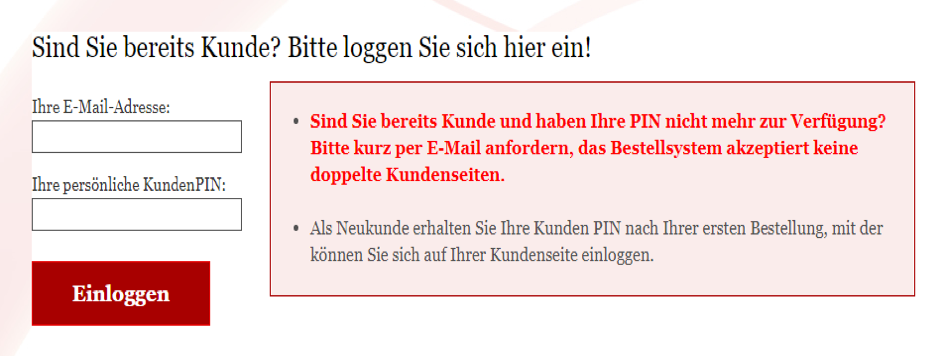
\includegraphics[width=0.7\linewidth]{Graphics/anmeldeformular.png}
	\caption[Anmeldeformular]{Die bisherige Eingabemaske für das Kundenlogin}
	\label{fig:anmeldeformular}
\end{figure}


\subsection{Registerformular}

Falls der Kunde keine PIN hat, muss er sich registrieren. Dieses Formular besteht aus fünf Abschnitten. Im ersten muss der Kunde seine persönlichen Daten angeben. Im zweiten steht die Informationen des Auftrags, darauf folgt die Menü-Auswahl und im vorletzten Schritt werden die Zubehör- und die Serviceauswahl angezeigt. Der letzte Abschnitt dient der Erklärung des Registrierungsprozesses. Die Abbildung \ref{fig:registerForm} gibt die Übersicht über Registerformular.

\begin{figure}
	\centering
	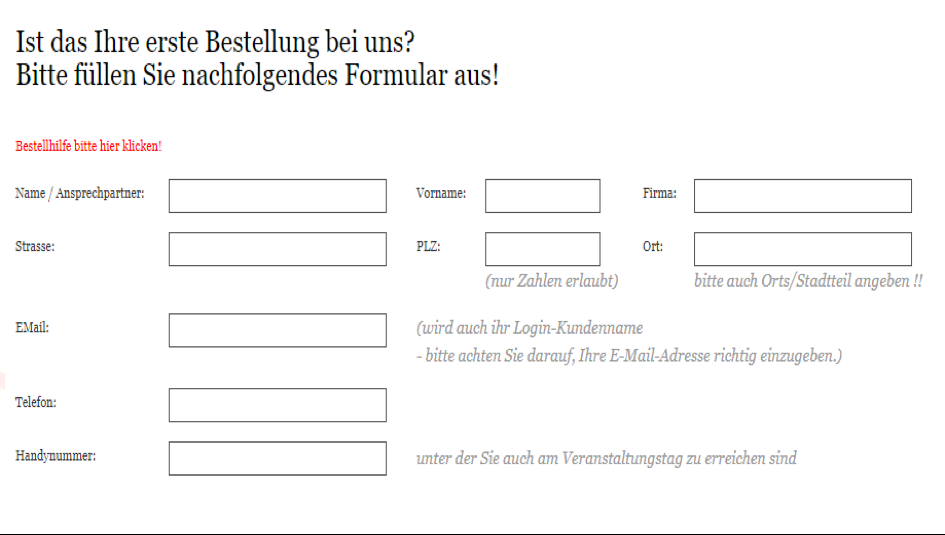
\includegraphics[width=0.7\linewidth]{Graphics/registerForm.png}
	\caption[Registerformular]{Die bisherige Eingabemaske für das Registrierungsformular}
	\label{fig:registerForm}
\end{figure}

\subsection{Auftraggeber-Verwaltung}

Im Fall einer Registeranfrage kann der Auftraggeber diese bestätigen oder löschen. Dem Auftraggeber stehen drei Optionen zur Verfügung: Auftragsverwaltung, E-Mail-Verwaltung und Umsatzverwaltung. Zuerst soll die Auftragsverwaltung betrachtet werden. Dort finden sich elf Optionen, neun davon leiten zu eigenen Unteroptionen weiter. Die anderen beiden sind „Speichern“ und „Abmelden“. Anhand dieser Optionen kann der Auftraggeber die Kundendaten einsehen, editieren, bearbeiten und löschen. Außerdem kann er die dazugehörigen Nachrichten lesen oder löschen. Auch kann er neue und alte Aufträge einsehen und bearbeiten oder löschen. Die Abbildung \ref{fig:Auftragverwaltung} zeigt die Ansicht der Auftraggeber-Verwaltung

\begin{figure}[h]
	\centering
	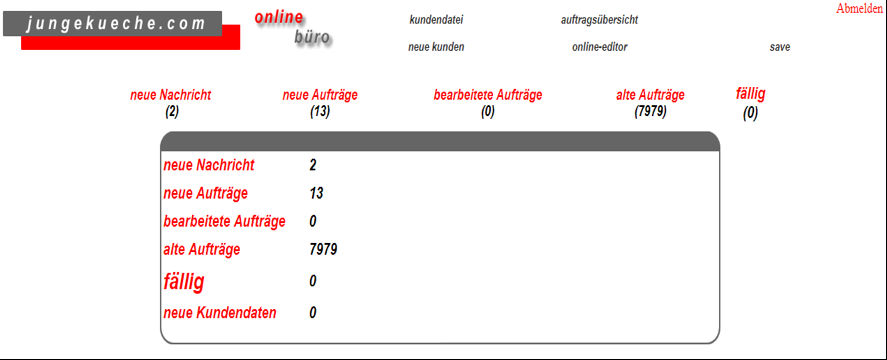
\includegraphics[width=0.7\linewidth]{Graphics/Auftragverwaltung.png}
	\caption[Auftragsverwaltung]{Die bisherige Eingabemaske für die Auftragsverwaltung}
	\label{fig:Auftragverwaltung}
\end{figure}

\subsection{Kundenansicht}

Wenn die Anfrage des Kunden bestätigt wird, erhält der Kunde einen PIN per E-Mail. Mit diesem PIN und seiner E-Mail kann der Kunde sich bei „jungekueche“ anmelden. Nach dem Login-Prozess gelangt er auf eine persönliche Nutzerseite. Dort findet er eine Übersicht über seine aktuellen und bisherigen Bestellungen, ein Kontaktfenster, in dem er Nachrichten einsehen oder schreiben kann, sowie eine Art Newsletter. Außerdem gibt es eine Option, über die der Kunde neue Bestellungen aufgeben kann. Abbildung \ref{fig:KundenAnsicht} veranschaulicht diese Ansicht. 

\begin{figure}[h]
	\centering
	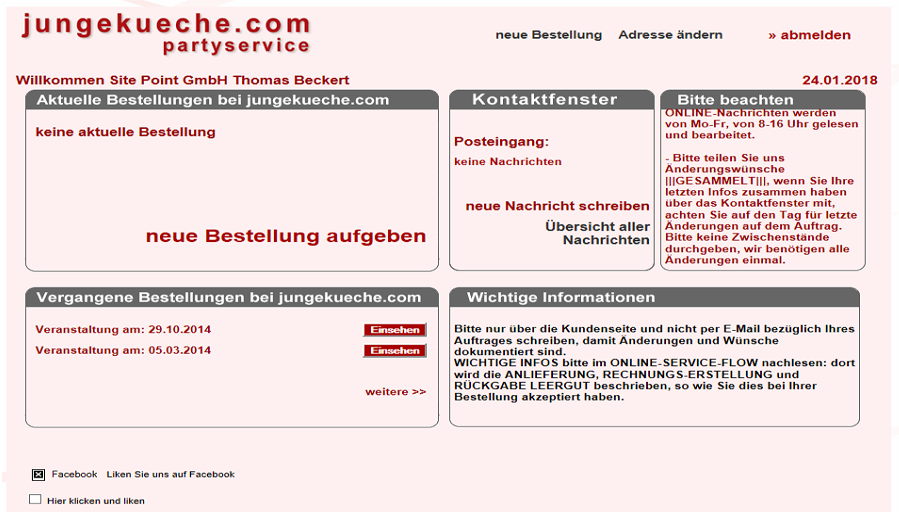
\includegraphics[width=0.7\linewidth]{Graphics/KundenAnsicht.png}
	\caption[Kundeansicht]{Die bisherige Eingabemaske für die Auftragsverwaltung}
	\label{fig:KundenAnsicht}
\end{figure}

\section{Beschreibung der Funktionalität}   

Einer Anmeldung muss immer eine Registrierung vorausgehen. Diese Funktionalität wird mit ASP und ASP.NET realisiert. Die verwendeten Hilfsprogramme sind JQuery, JavaScript, AJAX, HTML und CSS.
Zuerst wird betrachtet, wie die Kommunikation zwischen den verschiedenen Technologien funktioniert. Das ganze Programm besteht aus Front- und Backend. Das Frontend bezeichnet den Teil des Programms, den der Nutzer verwendet. Im Backend werden die Daten verarbeitet. Die Verbindung zwischen den beiden wird über JavaScript und JQuery realisiert. Wenn der Benutzer eine Tätigkeit ausführt, werden die eingegebenen Daten über JavaScript-Methoden zum Backend weitergeleitet. Dort werden sie verarbeitet und über die JavaScript-Methode aufgerufen. Dort werden sie bearbeitet und wieder zu dem Frontend zugeschickt. Das Backend entsteht aus ASP-Funktionen, in denen sich verschiedene Methoden sowie Datenbanken befinden. In den Datenbanken werden die eingegebenen Daten gespeichert. Ein Beispiel wird in der Abbildung \ref{fig:ASPArchitectur} dargestellt.

\begin{figure}[h]
	\centering
	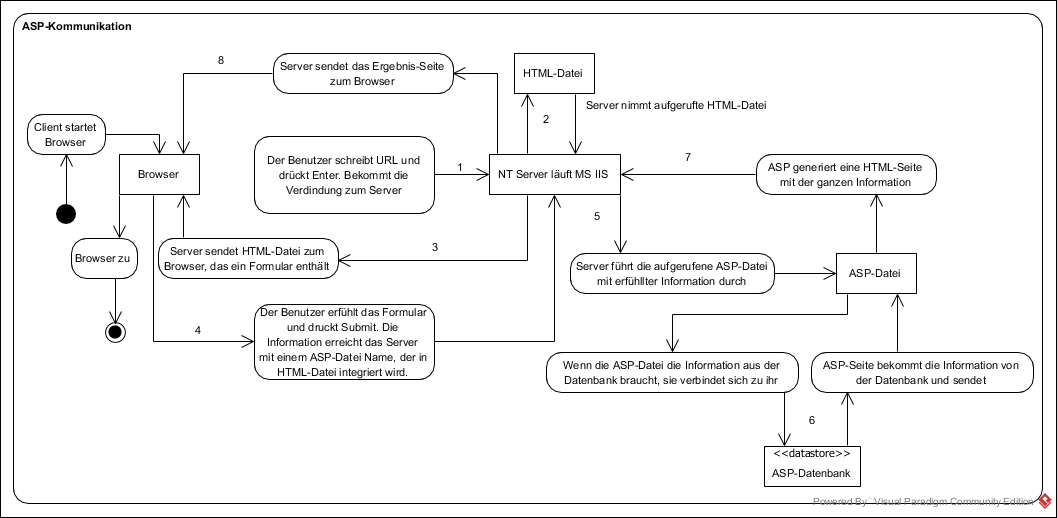
\includegraphics[width=0.9\linewidth]{Graphics/ASPArchitectur.png}
	\caption[ASPArchitectur]{ASP Architektur Model}
	\label{fig:ASPArchitectur}
\end{figure}

Nach der grundlegenden Kommunikation zwischen Front- und Backend, wird erläutert wie die einzelnen Kommunikationsabläufe zwischen Front- und Backend koordiniert werden.

\subsection{Anmelde- und Registerformular} 

Nach einem Klick auf das Feld „Bestellformular \& Login“ erscheinen das Anmeldeformular sowie die Bestellseite. Wenn der Kunde auf den Button „Anmeldung“ klickt, wird eine HTML-Post-Methode aktiviert. So werden zunächst JavaScript-Methoden aufgerufen. Diese werden benutzt, um die Eingabe auf Richtigkeit zu prüfen. Danach werden Methoden aus der ASP-Datei aufgerufen.
Das Registerformular funktioniert nach demselben Prinzip. Nach der Eingabe der benötigen Information werden diese geprüft. Bei einem korrekten Input werden die Eingaben zu den zugeordneten Daten bzw. Methoden geschickt. In der Abbildung \ref{fig:Bestellung} ist eine Übersicht über das Bestellformular zu sehen.

\begin{figure}[h]
	\centering
	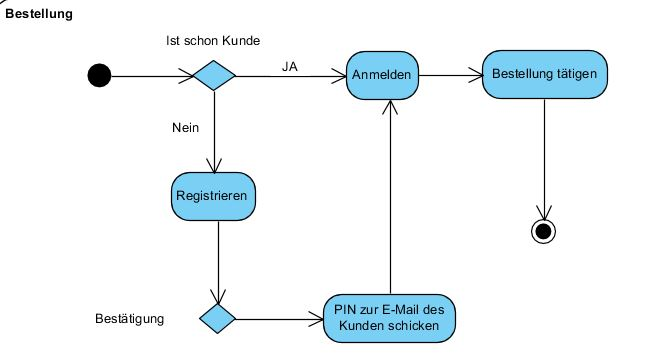
\includegraphics[width=0.9\linewidth]{Graphics/Bestellung.JPG}
	\caption[Anmeldung/Bestellung]{Die bisherige Eingabemaske für den Vorgang der Bestellung/Registrierung}
	\label{fig:Bestellung}
\end{figure}

\subsection{Auftraggeber-Verwaltung}

Die Auftragsverwaltung setzt sich, wie bereits beschrieben wurde, aus verschiedenen Optionen zusammen. Die Funktionsweise der jeweiligen Option soll im Folgenden separat betrachtet werden.
	
\subsubsection{Nachricht-Sektion} 

Sie ermöglicht dem Auftraggeber, die Information zu lesen oder zu löschen. Nach der zugeordneten Wahl wird die Information in der Datenbank „komentar“ entweder aufgerufen oder entfernt. In der Abbildung \ref{fig:lesenLoeschen} ist diese Aktivitäten zu sehen.

\begin{figure}[h]
	\centering
	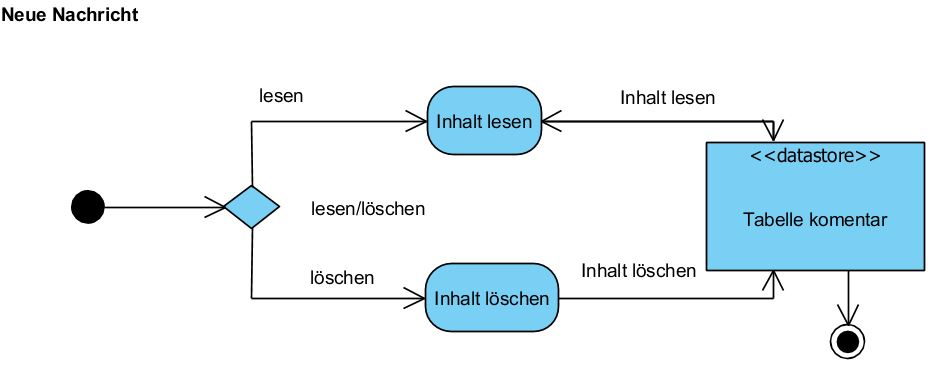
\includegraphics[width=0.8\linewidth]{Graphics/NeueNachricht.JPG}
	\caption[Kommunikation]{Die bisherige Eingabemaske für den Nachrichten lesen oder löschen}
	\label{fig:lesenLoeschen}
\end{figure}



\subsubsection{Aufträge: Neue, alte und bearbeitende}

Bei allen drei Arten von Aufträgen stehen identische Verwaltungsmöglichkeiten zur Verfügung. Der Auftraggeber kann den Auftrag sehen, editieren oder löschen. Jede dieser Aktivitäten ist mit mehreren Datenbanken verbunden, die verschiedene Informationen über die gewählten Artikel beinhalten. In der Abbildung \ref{fig:Autrag_Loeschen} wird zum Beispiel die Funktionalität ’löschen’ gezeigt. Es spielt keine Rolle, welche Art von Auftrag gewählt wird, denn die Funktionalität umfasst dieselben Datenbanken.

\begin{figure}[h]
	\centering
	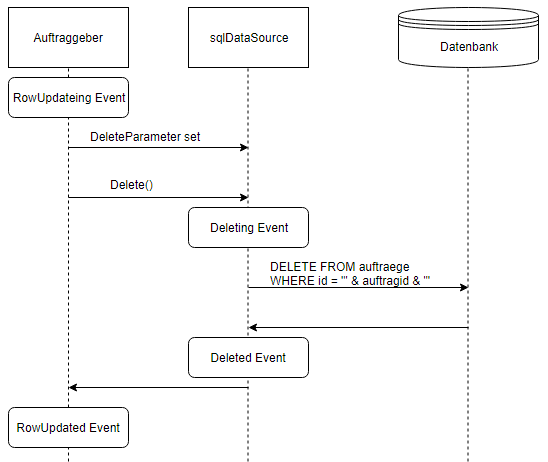
\includegraphics[width=0.6\linewidth]{Graphics/auftragLoeschen.png}
	\caption[AutragLoeschen]{Die bisherige Eingabemaske für den Auftrag löschen}
	\label{fig:Autrag_Loeschen}
\end{figure}

\pagebreak
\subsubsection{Kundendatei}

Hier befinden sich die Information über die Kunden. Es gibt die Möglichkeit, die Information zu editieren oder zu löschen. Um einen bestimmten Kunden schneller zu finden, steht eine Suchmaschine zur Verfügung. Eine Übersicht wird in der Abbildung \ref{fig:KundenDatei} dargestellt.

\begin{figure}[h]
	\centering
	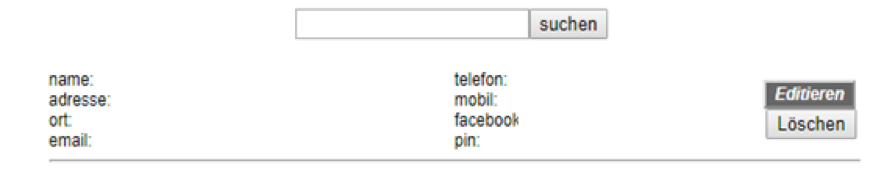
\includegraphics[width=0.7\linewidth]{Graphics/kundenDatei.png}
	\caption[Kundeansicht]{Die bisherige Eingabemaske für die Kundendatei}
	\label{fig:KundenDatei}
\end{figure}

Wenn man editieren oder löschen möchte, geschieht dies über die JavaScript-Funktion. Diese Funktion ruft die Methoden auf, die sich in der zugeordneten ASP-Datei befinden. Im „Editor-Fenster“ lassen sich die Daten des Kunden bearbeiten, Login-Daten wie E-Mails an Kunden übermitteln, wichtige Information für alle Kunden senden, es kann dem Kunden ein V.I.P-Status gegeben, es können spezifische Warnungen an den jeweiligen Kunden gegeben, Informationen geschrieben sowie Unterschriften editiert werden etc. Das Fenster wird in Abbildung \ref{fig:KundenEditor} gezeigt.

\pagebreak

\begin{figure}[h]
	\centering
	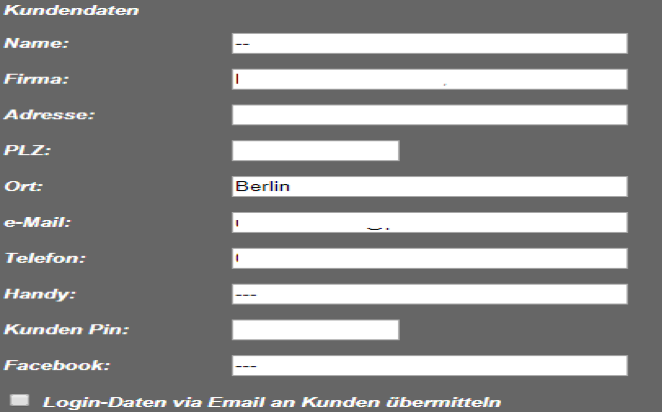
\includegraphics[width=0.7\linewidth]{Graphics/kundeEditieren.png}
	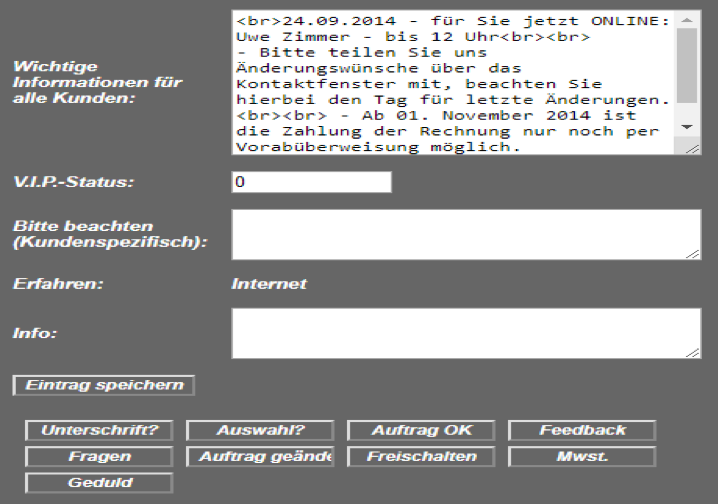
\includegraphics[width=0.7\linewidth]{Graphics/kundeEditieren1.png}
	\caption[Kundeansicht]{Die bisherige Eingabemaske für das Kunden-Editor}
	\label{fig:KundenEditor}
\end{figure}

Durch JavaScript-Methoden wird eine zusätzliche Möglichkeit generiert, neue Nach-richten an dem Kunden zu schreiben. Sie wird aktiviert, wenn in der Liste des Adressbuchs mit dem Cursor über den Namen eines bestimmten Kunden gefahren wird. Die Kommunikation zwischen dem Auftraggeber und dem Kunden wird auch in der Datenbank „komentar“ gespeichert.

\subsubsection{Online-Editor}

Mit dieser Option können neue Artikel erstellt, editiert und gelöscht werden. Es gibt „Artikel-Arrangements“ und „Artikel-Standard“. Bereits erstellte Artikel können entweder gelöscht, editiert oder zugeordnet werden. JavaScript-Funktionen werden verwendet, um die Eingaben zu prüfen. Wenn die Eingaben korrekt ausgefüllt worden sind, werden die obengenannten Methoden aus den jeweiligen Dateien aufgerufen. In der folgenden Abbildung \ref{fig: Online-EditorUebersicht} ist eine Übersicht über die Seite zu sehen.

\pagebreak

\begin{figure}[h]
	\centering
	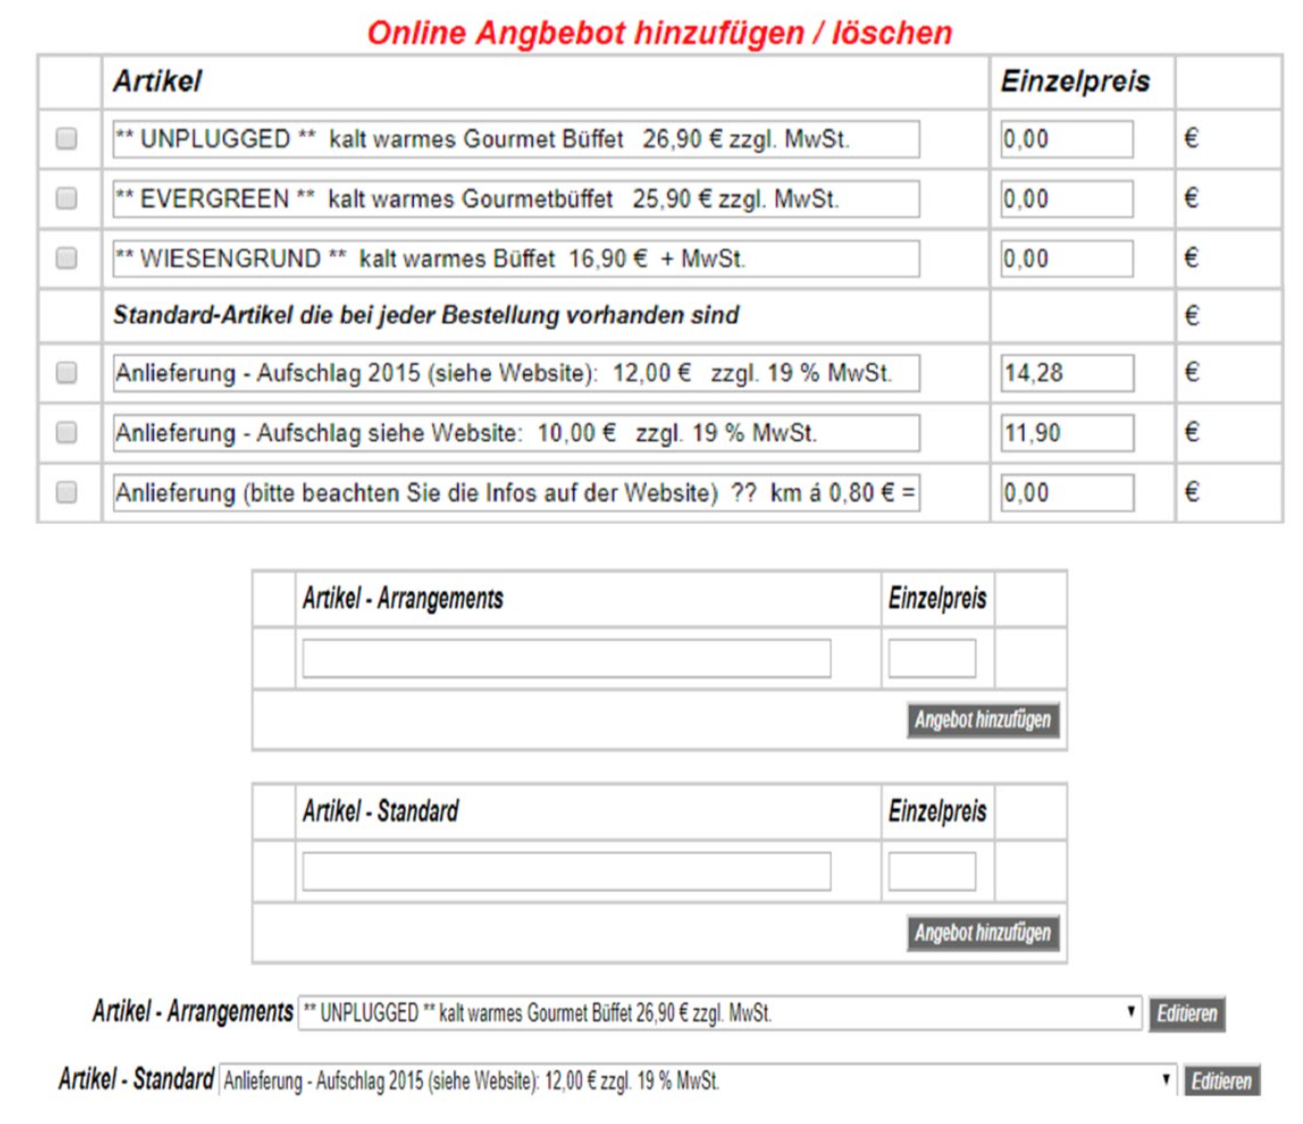
\includegraphics[width=0.7\linewidth]{Graphics/menue-uebesicht.png}
	\caption[Kundeansicht]{Die bisherige Eingabemaske für die Übersicht das Menü}
	\label{fig: Online-EditorUebersicht}
\end{figure}

Wenn die Option „Editieren“ zu den „Artikel-Arrangements“ ausgewählt wird, wird eine neue Seite geöffnet, in der es verschiedene Möglichkeiten gibt, die Inhalte und Daten zu bearbeiten. Abbildung \ref{fig: Editor-Menü2} zeigt diese Seite.
Bei „Artikel-Standard“ gibt es nur eine Möglichkeit. Sie wird in der Abbildung \ref{fig: Editor-Menü-Standard} dargestellt.

\begin{figure}[h]
	\centering
	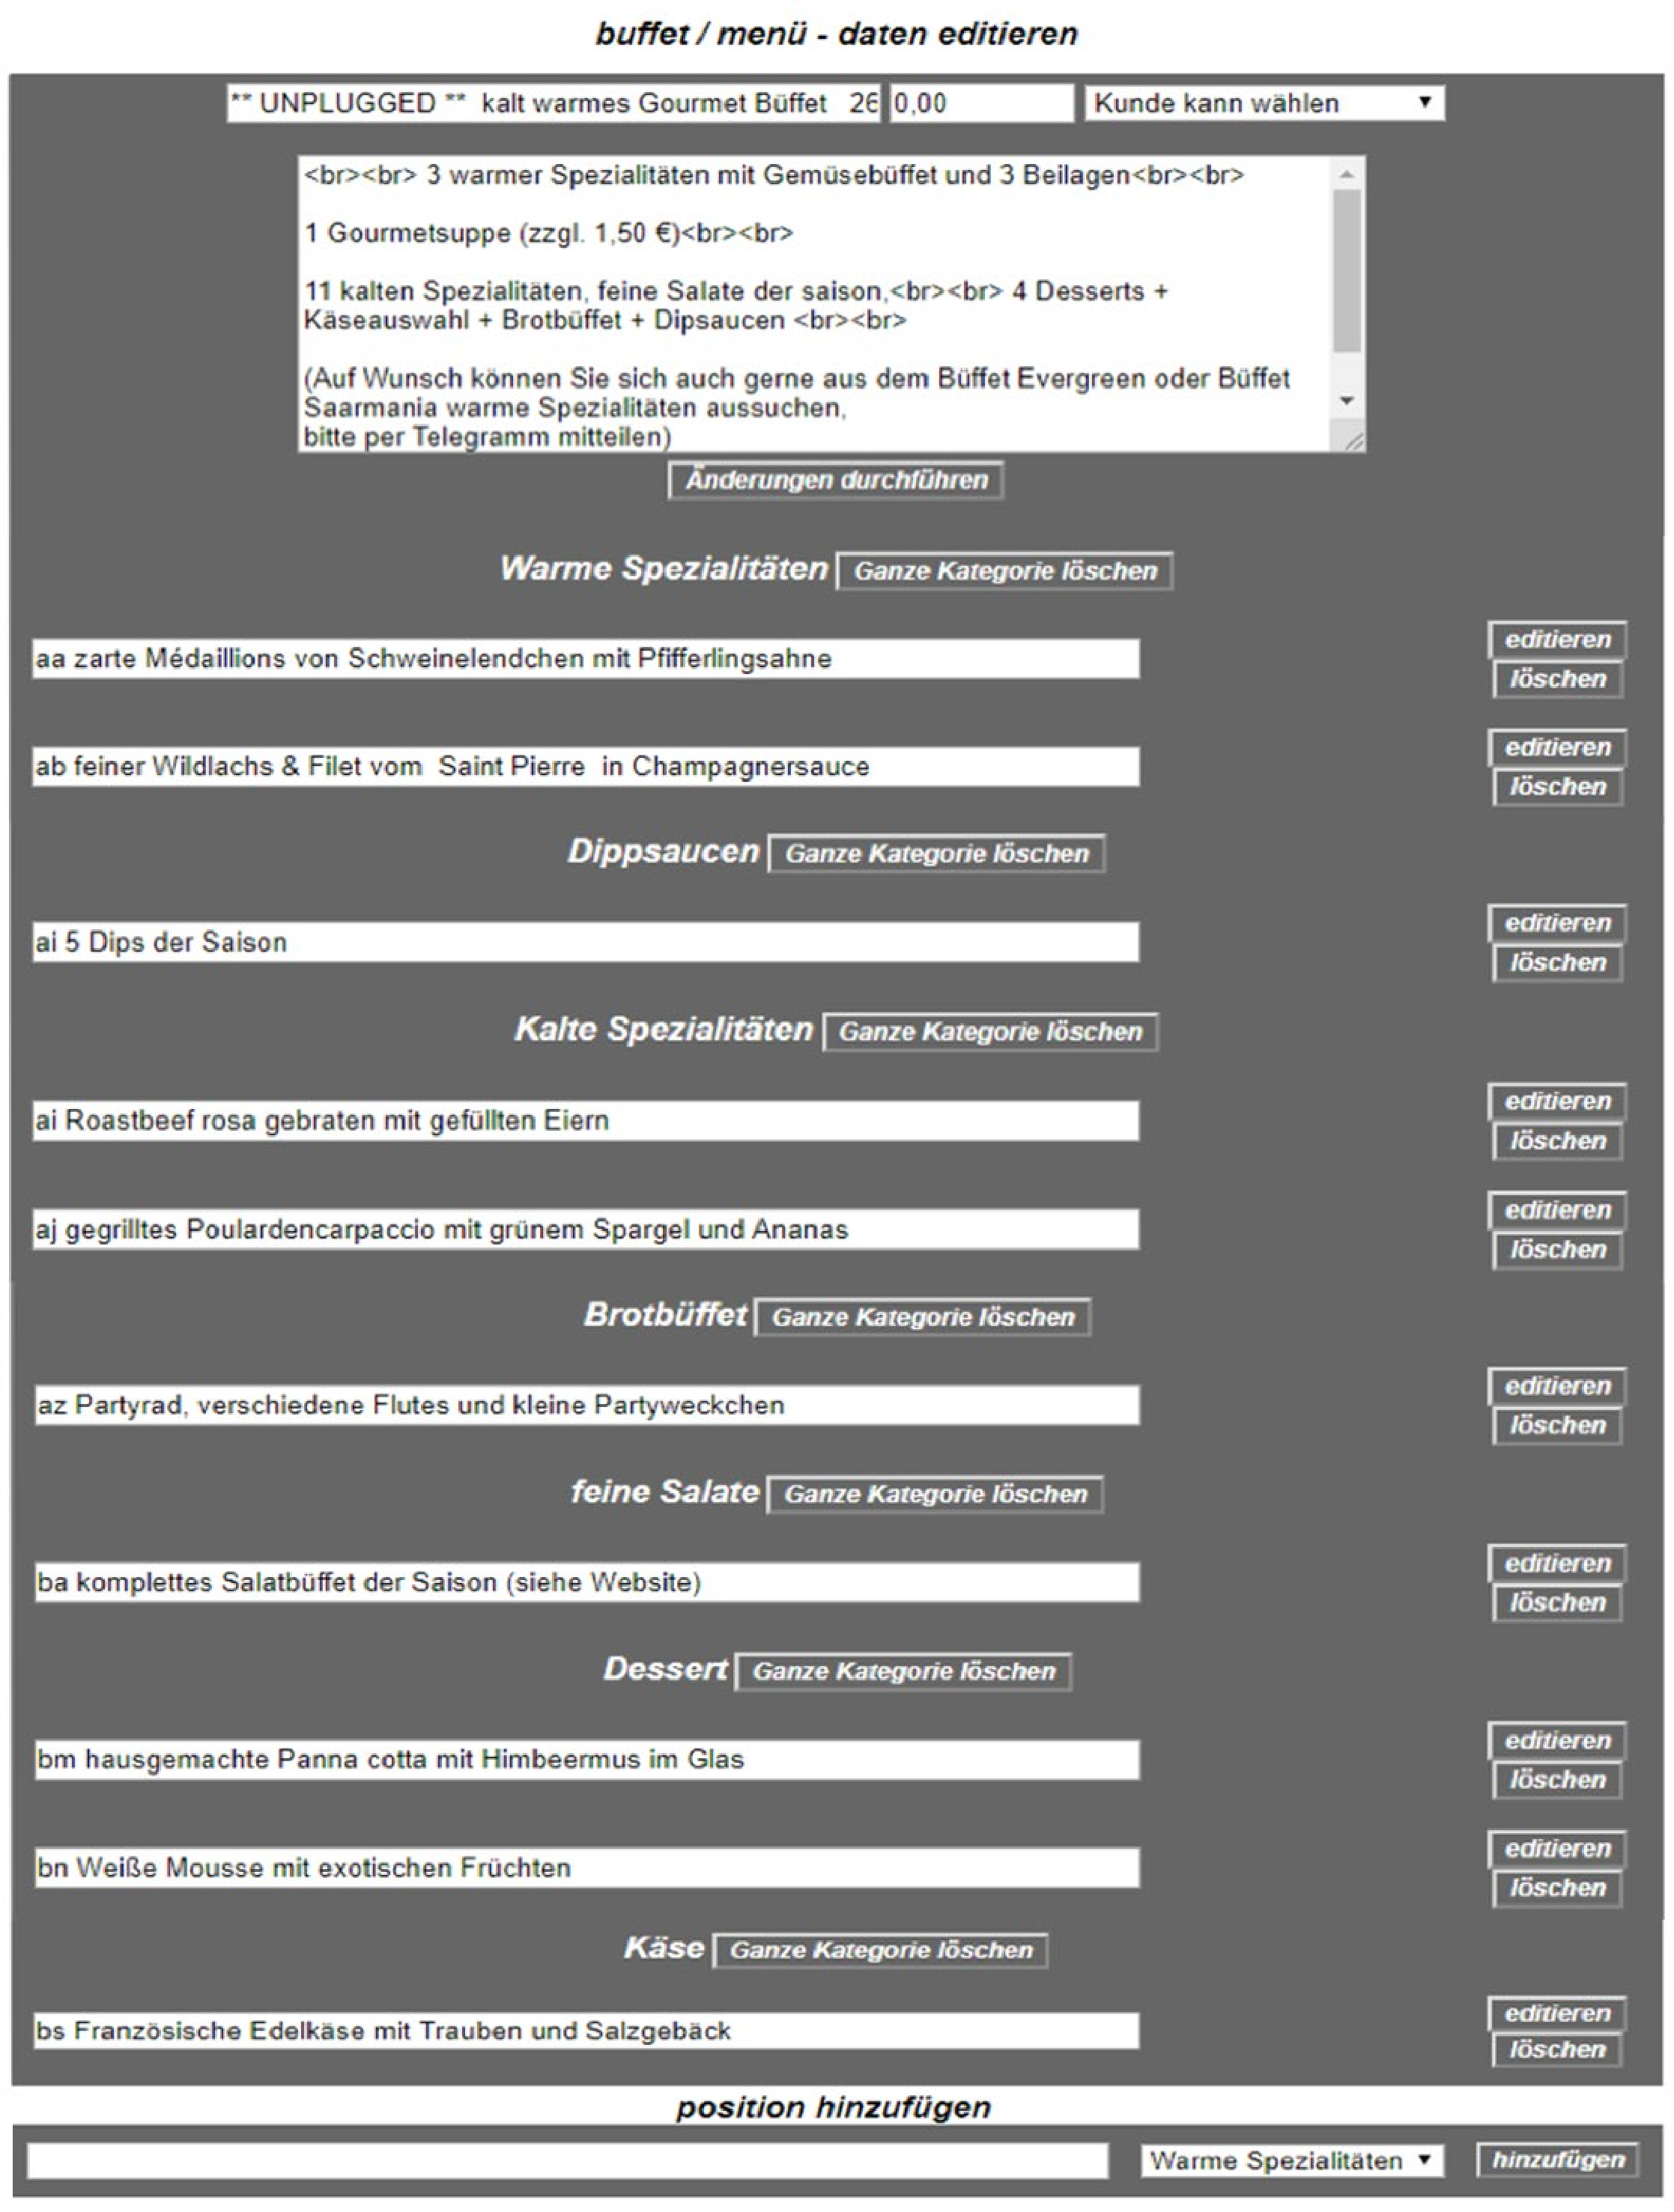
\includegraphics[width=0.7\linewidth]{Graphics/arrangement-Menue-editor.pdf}
		\caption[Kun2deansicht]{Die bisherige Eingabemaske für die Übersicht des Menü-Editor-Arrangements}
	\label{fig: Editor-Menü2}
\end{figure}

\begin{figure}[h]
	\centering
	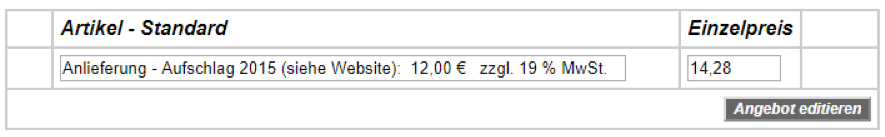
\includegraphics[width=0.7\linewidth]{Graphics/menuStandart.png}
	\caption[Kundeansicht]{Die bisherige Eingabemaske für die Übersicht des Menü-Editor-Standard}
	\label{fig: Editor-Menü-Standard}
\end{figure}


\section{Testen} 

Für diese Arbeit wird ein webbasierter Sicherheit-Checker von 1\&1 verwendet. Eine grundlegende Recherche hat gezeigt, dass die Webseite auf einer mittleren Sicherheitsstufe steht. Die Webseite ist nach vier Kriterien ohne Beanstandung abgesichert.

\begin{itemize}	
	
\item\ac{SSL} Verschlüsselung – Über SSL wird sichergestellt, dass zwischen User und Server die übertragenen Daten nicht gelesen werden können.

\item Cookies sind auch sicher und so ist der Browser von Dritten über JavaScript unlesbar.

\item Apache-Status ist verboten. Die Status-Seite ist öffentlich nicht erreichbar. So wird den Schutz von potenziellen Angreifern erhöht. 

\item Die Server Version ist öffentlich nicht einsehbar. Damit kann ein Angreifer nicht einfach bekannte Schwachstellen ausnutzen.
\end{itemize}

\begin{figure}[h]
	\centering
	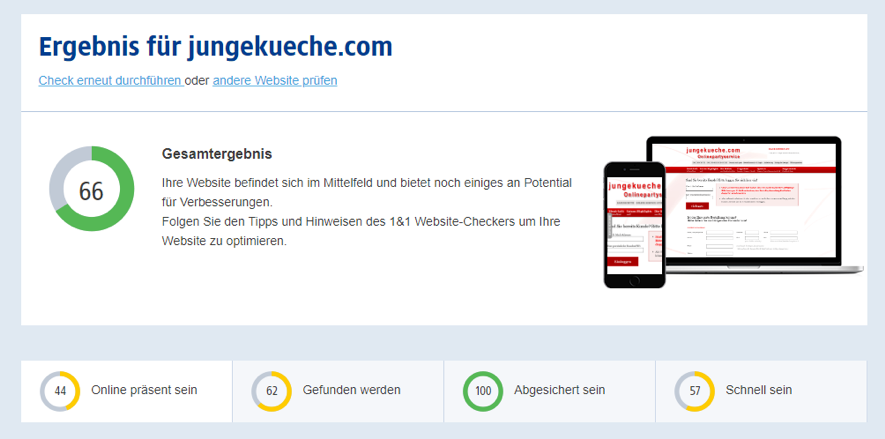
\includegraphics[width=1\linewidth]{Graphics/egebnis1to1.png}
	\caption[Egebniss Von 1zu1]{Ergebnis vom 1zu1}
	\label{fig: ErgebnissVonEinZuEin}
\end{figure}

Wie die Abbildung \ref{fig: ErgebnissVonEinZuEin} zeigt, ist die Webseite gesichert, aber es gibt einige Bereiche, die eine Optimierung benötigen würden. Die Seite lädt langsam, wird im Browser relativ oft gefunden, aber ist sie gesichert.
Über einen anderen Web-Checker werden weitere Funktionalitäten der Webseite analysiert. Observatory \cite{King2018} von Mozilla analysiert den Browser im vier Schritten.

\begin{itemize}	
	\item \ac{HTTP}
	\item \ac{TLS}
	\item \ac{SSH}
	\item Third-Party Tests
\end{itemize}

Hier werden nur die ersten beiden Schritte betrachtet, da nur sie für diese Arbeit relevant sind.

\pagebreak

\textbf{HTTP Observatory}

Hier wird die aktuelle Sicherheit der Webseite im öffentlichen Internet betrachtet. Alle Anfragen werden über POST- oder GET-Methoden durchgeführt und die Rückmeldungen erfolgen im JSON-Format. In dieser Analyse wird gezeigt, dass \ac{CSP}nicht implementiert wurde. CSP verhindert Weitbereich von \ac{XSS}- und „clickjacking“-Attacken. Cookes sind teilweise gesichert. Hier fehlen das „Secure“-Attribut sowie „SameSite“ und „Prefix“. Durch „Secure“ werden die Cookies davon abgehalten, dass sie über nicht gesichertes HTTP versendet werden. „SameSite“ hält die Cookies von \ac{CSRF}-Attacken und Cross-Site-Übersendung ab, d. h. es ist nicht auszuschließen, dass ein Hacker-Angriff auf das Computersystem des Benutzers erfolgt. Es werden keine \_Host- und \_Secure-Prefixe auf den Namen der Cookies verwendet. Das bedeutet, dass sie nicht gegen Überschreiben geschützt sind. Die Abbildung \ref{fig: HTTP Observatory: Ergebnis} zeigt die genaue Bewertung der Webseite mit dem Resultat der durchgeführten Analyse.
 
\begin{figure}[h]
	\centering
	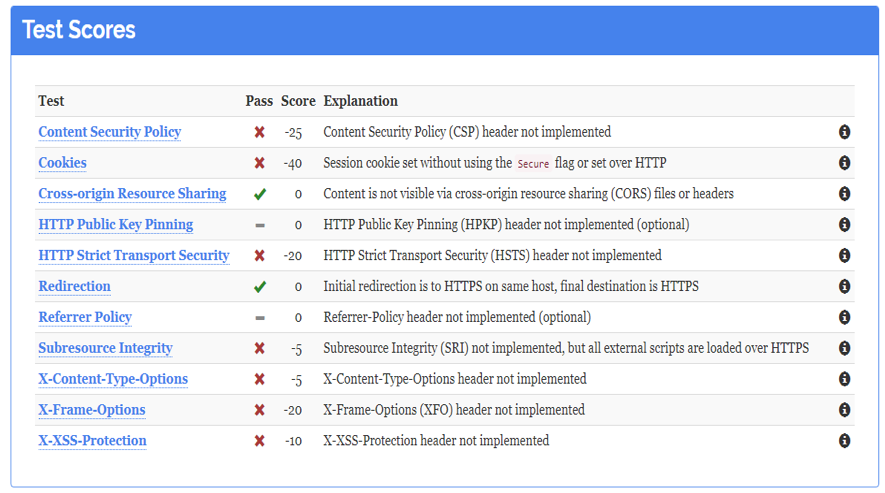
\includegraphics[width=0.7\linewidth]{Graphics/eergebnisobser.png}
	\caption[Egebniss vom HTTP Observatory]{ Ergebnis vom HTTP Observatory }
	\label{fig: HTTP Observatory: Ergebnis}
\end{figure}

\textbf{TLS}

Die hier betrachtete Webseite verwendet das Signaturverfahren SHA-256-With-RSA. Das bedeutet, dass eine Kombination zwischen SHA256 (kryptologische Hashfunktion,

die Hashwerte mit einer Länge zwischen 256 und 512 Bits erzeugt) und \ac{RSA} (dadurch können symmetrische Schlüssel jeder üblichen Länge erzeugt werden) vorliegt (siehe Abbildung \ref{fig: TSL Observatory: Ergebnis}).

\begin{figure}[h]
	\centering
	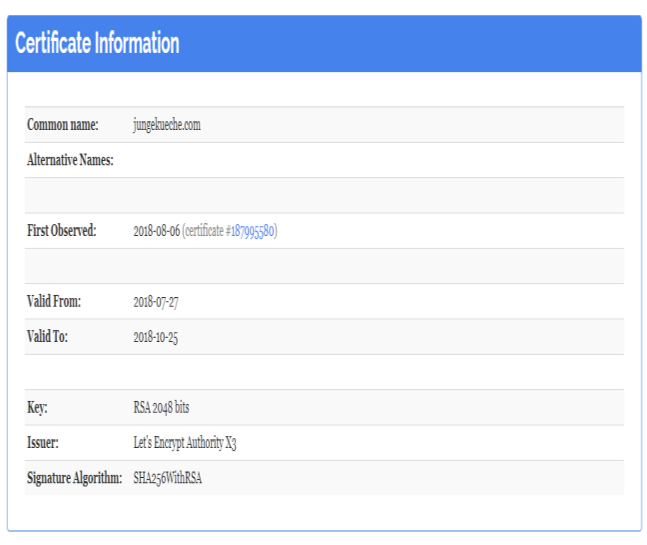
\includegraphics[width=0.6\linewidth]{Graphics/obser2.png}
	\caption[Egebniss TSL Observatory]{Ergebnis vom TLS Observatory}
	\label{fig: TSL Observatory: Ergebnis}
\end{figure}

\section{Warum ist eine Migration notwendig?}

ASP ist eine nicht Objekt-Orientierte Skripte Sprache. Es ist anfällig zu Unterbrechung der Applikationen, z. B. wenn die \ac{IIS} gestoppt und neu gestartet werden. Wenn eine ASP-Seite aufgerufen wird, wird der Text linear analysiert. Die Frontend-Verwendung des Bestellsystems ist verschachtelt und es gibt redundante Optionen. Das Login- und Registrierungs-Menü sowie das Bestellformular befinden sich auf einer Seite. Dadurch wird das Öffnen der Seite verlangsamt. Es gibt unnötigen Quellcode, der entfernt werden kann. Ein anderer Nachteil des Systems ist, dass es nicht dynamisch orientiert ist, d. h. die Umgebung ist nicht benutzerfreundlich. Der Auftraggeber muss für jede nötige Änderung den Entwickler kontaktieren. Dadurch ist der Benutzer vom Hersteller des Programms abhängig. Aktuell gibt es eine große Auswahl an CMS, durch die dem Auftragsgeber zahlreiche Möglichkeiten für Änderungen seiner Website zur Verfügung stehen. Im folgenden Kapitel wird eines dieser CMS erläutert.




